%@@@@@@@@@@@@@@@@@@@@@@@@@@@@@@
%@@@@@@@@@ Usepackage @@@@@@@@@
%@@@@@@@@@@@@@@@@@@@@@@@@@@@@@@
\documentclass{beamer}

%\usetheme{Madrid}
%\usecolortheme{beaver}

% setting margin
%\usepackage[a4paper,left=0.5in,right=0.5in]{geometry}
% color package
\usepackage{xcolor}
% tablur combine
\usepackage{multirow}

%--------------------
%-- define comment --
%--------------------
%\long\def\/*#1*/{}
%__ define comment __
%____________________

%------------------
%-- math package --
%------------------
\usepackage{amssymb,amsmath,stmaryrd} 
%------------------
\usepackage{mathtools}
%Reference: 
%http://texdoc.net/texmf-dist/doc/latex/mathtools/mathtools.pdf
%__ math package __
%__________________


%------------------------------------
%-- insert {} to multiple folders ---
%------------------------------------
\usepackage{graphicx}
\graphicspath{{./images/},{./image/}} 
%__ insert {} to multiple folders ___
%____________________________________


%------------------
%-- use chinese ---
%------------------
\usepackage{CJKutf8}
%__ use chinese ___
%__________________

%----------------------
%-- use draw package --
%----------------------
\usepackage{tikz}
%__ use draw package __
%______________________


%----------
%-- url ---
%----------
\usepackage{hyperref}
% sample
% \url{http://...}
% \href{http://...}{text hyperlink}
%__ url ___
%__________

%----------------
%-- underline ---
%----------------
\usepackage{soul}
% using with
% ul{...}
%__ underline ___
%________________

%----------------------
%-- background color --
%----------------------
\usepackage{lipsum}
\usepackage[most]{tcolorbox}
\definecolor{bg}{RGB}{255,249,227}
\definecolor{block_green}{RGB}{203,247,235}
%__ background color __
%______________________

%----------
%-- code --
%----------
\usepackage{listings}
%__ code __
%__________

%@@@@@@@@@@@@@@@@@@@@@@@@@@@@@@@@@@@@@@@@@@@@@@@@
%@@@@@@@@@@@@@@ Enumerate command @@@@@@@@@@@@@@@
%@@@@@@@@@@@@@@@@@@@@@@@@@@@@@@@@@@@@@@@@@@@@@@@@
\makeatletter
\newcommand\setItemnumber[1]{\setcounter{enum\romannumeral\@enumdepth}{\numexpr#1-1\relax}}
\makeatother

% command
%\setItemnumber{5}
%============== Enumerate command ===============
%================================================

%--------------------
% -- Merge pdf ------
\usepackage{pdfpages}

%\includepdf[pages=-]{paper1}

%--------------------
%--------------------

%----------------------------------------   multiple columns
\usepackage{multicol}

% begin{multicols}{2}
%
% end{multicols}
%---------------------
%------------------------------------------------------------
%
%               multiple divide add substract 
%
%------------------------------------------------------------
% add multiple
\usepackage{xlop}

% \opmul{384}{56}
% \opadd{1234}{567}

% divide
\usepackage{polynom}

% \input{longdiv}
% \longdiv{12345}{13}
%
%______________ multiple divide add substract _______________
%____________________________________________________________

%--------------------   font
%\usepackage{lmodern}
\usepackage[T1]{fontenc}


%========= Usepackage =========
%==============================

%@@@@@@@@@@@@@@@@@@@@@@@@@@@@
%@@@@@@@@@ Document @@@@@@@@@
%@@@@@@@@@@@@@@@@@@@@@@@@@@@@
\title{\textbf{}}
\author{\textbf{sjLin}}
%\date{}
%------------
%-- Start ---
%------------
\begin{document}

{\fontfamily{lmss}\selectfont
% bsmi
\begin{CJK*}{UTF8}{bkai}

%\maketitle

%__ Start ___
%____________




\begin{frame}
\frametitle{判斷有理數}
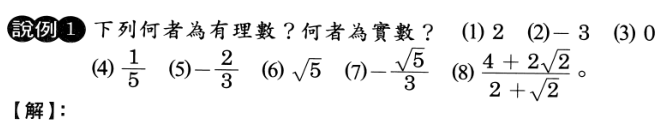
\includegraphics[width=\textwidth]{ex1.png}
\begin{itemize}
 \item 
有理數: 可以分成兩整數形式的分數。\\
所以有 2, -3, 0, $\frac{1}{5}$, $-\frac{2}{5}$,\\
$
\frac{4+2\sqrt{2}}{2+\sqrt{2}}
$
$\cdot$
$
\frac{2-\sqrt{2}}{2-\sqrt{2}}
$
$=
\frac{8-4\sqrt{2}+4\sqrt{2}-4}{4-2}
$
$= 2$

 \item
實數為不含虛數之值, 以上皆為實數。


\end{itemize}

\end{frame}

\begin{frame}
 \frametitle{有理數+無理數} 

\includegraphics[width=\textwidth]{real_null}
\begin{enumerate}
 \item 
$
a-c=(d-b)\sqrt{e}
$, 假設$(d-b)$不為零,\\
則$\sqrt{e}=\frac{a-c}{d-b}$為有理數矛盾。 \\[0.5cm]
假設$(d-b)$為零, 即$b=d$, $a-c=0\cdot \sqrt{e}\Rightarrow a=c$

\item
策略: 找一反例, 有反例則答案為否。\\
$(a,\;b,\;c,\;d)=(1,\;2,\;1+\sqrt{2},\; \sqrt{2})$
\end{enumerate}
\end{frame}
\begin{frame}
 
\includegraphics[width=\textwidth]{ex3}
 $
 2x+\sqrt{5}x+y-\sqrt{5}y
 =
 8-2\sqrt{5}
 $\\
 等式整理
 $\Rightarrow (2x+y-8)+(x-y+2)\sqrt{5}=0$\\
 $\Rightarrow (x-y+2)=0$, 否則$\sqrt{5}=\frac{(2x+y-8)}{(x-y+2)}$為有理數矛盾。
 \\
 $
 \begin{cases}
  2x+y &=8\\
  x-y  &=-2
 \end{cases}
 $\\[0.5cm]
 $\Rightarrow (x,\;y)=(2,\;4)$
\end{frame}

\begin{frame}
 \frametitle{有理數 - 直接證法}
 
\includegraphics[width=\textwidth]{ex4}
 \begin{itemize}
  \item 
$
\begin{cases}
 3a+2b &= p \\
 2a-b  &= q
\end{cases}
\Rightarrow p,q\in \mathbb{Q}
$\\
計算$(a,b)$, 形式要是$p,q$組成\\
計算$b$\\ 
$
a+3b=(p-q) \Rightarrow a = (p-q)-3b
$代入第二式\\
$
2p-2q-6b-b = q \Rightarrow 2p-3q = 7b \Rightarrow b = \frac{2p-3q}{7}
$ \\ 
計算$a$, 由第二式變換 \\
$
a = \frac{q+b}{2}
$代剛得出來的$b$\\
$
a=
\frac{1}{2}\cdot \frac{2p+4q}{7}
=
\frac{p+2q}{7}
$
 \end{itemize}
\end{frame}

\begin{frame}
 \begin{itemize}
  \item 
 $\because  p\in \mathbb{Q}, q\in \mathbb{Q}, 2q\in \mathbb{Q}$
 $\Rightarrow p+2q\in \mathbb{Q} \Rightarrow \frac{p+2q}{7}\in \mathbb{Q}$
 \\$\therefore a\in \mathbb{Q}$
 \\[0.5cm]
 $\because 2p\in \mathbb{Q}, 3q\in \mathbb{Q}$
 $\Rightarrow 2p-3q \in \mathbb{Q}$
 $\Rightarrow \frac{2p-3q}{7}\in \mathbb{Q}$
 \\
 $\therefore b\in \mathbb{Q}$


\item
 $3a+2b$ , $2a-b$ $\in\mathbb{Q}$\\
 Pf. $(3a+2b)+(2a-b)\in\mathbb{Q}$ \\
 $\because a, b\in \mathbb{Q} $\\
 $\therefore 5a+b\in\mathbb{Q}$

 \end{itemize}

 
\end{frame}




%------------
%-- Finish --
%------------
\end{CJK*}
}
\end{document}
%__ Finish __
%____________

%========= Document =========
%============================
